% CVPR 2023 Paper Template
\documentclass[10pt,twocolumn,letterpaper]{article}

\usepackage[review]{cvpr}
\usepackage{graphicx}
\usepackage{amsmath}
\usepackage{amssymb}
\usepackage{booktabs}
\usepackage{xcolor}
\usepackage{placeins}
\definecolor{updateblue}{rgb}{0.0, 0.2, 0.75}

\usepackage[pagebackref,breaklinks,colorlinks]{hyperref}
\usepackage[capitalize]{cleveref}

\crefname{section}{Sec.}{Secs.}
\Crefname{section}{Section}{Sections}
\Crefname{table}{Table}{Tables}
\crefname{table}{Tab.}{Tabs.}

\def\cvprPaperID{02}
\def\confName{EE2000}
\def\confYear{2026}

\begin{document}

%%%%%%%%% TITLE
\title{FPGA-Based Underwater Image Color Correction Engine\\
\large{Hardware Implementation of Color Balance and Fusion on AMD Spartan-7}}

\author{
  [Author Name]\\
  Department of Electronics and Communication Engineering\\
  [Institution Name]\\
  {\tt\small [email@institution.edu]}
}
\maketitle

%%%%%%%%% ABSTRACT
\begin{abstract}
  A common issue arising in the case of underwater photographs is the presence of a blue-green cast over the image and loss of sharpness and clarity. This is due to the absorption of red wavelengths by water, and uneven scattering of different colors of light. Several methods have been formulated to enhance such photographs, but have fallen short either due to long computation times or high hardware costs. In this work, we present an FPGA-based hardware implementation of the Color Balance and Fusion algorithm proposed by Ancuti \emph{et al.}~\cite{ancuti2018color} on an AMD Spartan-7 FPGA (Boolean Board). The system loads the photograph onto the BRAM of the FPGA and produces a perceptually correct, contrast-enhanced image through a three-stage hardware pipeline:(1) White balance of the image is restored through red-channel re-compensation. (2)  Two enhanced inputs are derived via gamma correction and normalised unsharp masking. (3) Quality-map based fusion of the two inputs is done to create the final, enhanced image. The final image is streamed to the host PC via UART for metric evaluation. The proposed hardware engine demonstrates that the complete Ancuti 2018 pipeline can be realized entirely without a CPU, with all pixel arithmetic implemented as fixed-point operations in Verilog RTL, making it a cost-effective and suitable solution for edge deployment in bandwidth- and power-limited marine environments.
\end{abstract}

%%%%%%%%% BODY TEXT
\section{Introduction}
\label{sec:intro}

Underwater imaging is crucial for a wide range of marine science and
engineering applications, including autonomous underwater vehicle (AUV)
navigation, coral reef monitoring, pipeline and underwater cable inspection, and archaeological
surveying. However, images captured underwater are inherently degraded.
The absorption of light by water is wavelength-dependent: red light
(wavelengths $\sim$620--750\,nm) is absorbed within the first 1--2 meters
of depth, orange within 4--5 meters, and yellow within 8--10 meters, leaving
only the blue-green spectrum at greater depths. Additionally, light
scattered by suspended particles reduces contrast and produces a hazy veil.

Traditional enhancement methods such as histogram equalization or white
balance alone are insufficient for such combined multiplicative and additive
degradation. State-of-the-art software algorithms~\cite{ancuti2018color,
peng2017underwater, galdran2015automatic} have demonstrated excellent results,
but run on general-purpose CPUs or GPUs. In edge-deployed marine systems,
a dedicated hardware accelerator offers significant advantages: deterministic
latency, low power consumption, and elimination of the much more costly general-purpose CPU alternative.

We propose an FPGA implementation of the Color Balance and Fusion
algorithm~\cite{ancuti2018color}, by making use of the AMD Spartan-7 on the
Real Digital Boolean Board. The algorithm is chosen because every
stage---red-channel compensation, Gray World white balance, gamma LUT, and
unsharp masking---maps cleanly onto FPGA primitives (accumulators, DSP
slices, Block RAM LUTs, and shift registers), making it the most
hardware-friendly high-quality underwater enhancement algorithm available.
Images are processed offline from Block RAM and results are evaluated against
the UIEB benchmark~\cite{li2020underwater} using UCIQE~\cite{yang2015uciqe}
and UIQM~\cite{panetta2016uiqm} metrics computed on a host PC.

Applications of this protocol include:
\begin{itemize}
    \item \textbf{Image dehazing}. Dehazing refers to the removal of haze and fog in the original images, introduced by back scattering of light coming from the camera's flash and the forward scattering of natural light reflected off of the object's surface. 
    \item \textbf{Increased accuracy of object tracking and image matching.} This is due to the increased contrast in the enhanced image, and the non-introduction of artifacts in the enhanced image.
    \item \textbf{Increased accuracy of segmentation in images}, due to better boundary perception. Segmentation is the process of dividing an image into discrete and homogenous regions on the basis of some observable characteristic like texture, color, etc. 
\end{itemize}


\section{Related Work}
\label{sec:related}

Underwater image enhancement approaches can be broadly categorized into
physical model-based methods and non-physical model-based methods.

\subsection{Physical Model-Based Methods}

Physical model-based approaches treat enhancement as an inverse problem over
the simplified underwater image formation model:
\begin{equation}
  I(x) = J(x)\,e^{-\eta d(x)} + B_\infty(x)\!\left(1 - e^{-\eta d(x)}\right)
  \label{eq:ifm}
\end{equation}
where $I(x)$ is the observed degraded image, $J(x)$ is the scene radiance
to recover, $d(x)$ is depth, $\eta$ is the attenuation coefficient, and
$B_\infty(x)$ is the back-scattered ambient light (analogous to air-light in
outdoor haze). The goal is to estimate the transmission $t(x) = e^{-\eta d(x)}$
and ambient light $B_\infty$ and then invert \cref{eq:ifm}.

Galdran \emph{et al.}~\cite{galdran2015automatic} proposed the Red Channel
Prior, observing that because red light attenuates fastest, the reciprocal
of the red channel $(1-J^R)$ behaves like the dark channel of He
\emph{et al.}~\cite{he2009dark} in outdoor haze. They define:
\begin{equation}
  \begin{aligned}
    J^{RED}(x) &:= \min\!\Biggl(\min_{y\in\Omega(x)}\bigl(1-J^R(y)\bigr), \\
    &\qquad \min_{y\in\Omega(x)} J^G(y), \, \min_{y\in\Omega(x)} J^B(y)\Biggr) \approx 0
  \end{aligned}
  \label{eq:redchannel}
\end{equation}
which allows transmission estimation and scene recovery without manual
parameter specification, handling artificially illuminated scenes gracefully
via an added saturation prior.

Peng and Cosman~\cite{peng2017underwater} further improve depth estimation
by combining three complementary cues---the red channel map, the maximum
intensity prior (MIP), and image blurriness---through a sigmoid-weighted
combination:
\begin{equation}
  \begin{aligned}
    \widetilde{d_n}(x) &= \theta_b\!\left[\theta_a\,\widetilde{d_D}(x)
    + (1-\theta_a)\,\widetilde{d_R}(x)\right] \\
    &\quad + (1-\theta_b)\,\widetilde{d_B}(x)
  \end{aligned}
  \label{eq:peng_depth}
\end{equation}
where $\theta_a$ and $\theta_b$ are sigmoid functions of background light
brightness and average red content, respectively. The per-channel
transmission maps follow Beer--Lambert attenuation,
$t^c(x) = e^{-\beta^c d(x)}$, where the attenuation coefficients $\beta^c$
differ across the red, green, and blue channels.

While these physical model-based methods are theoretically grounded,
they require complex operations---local minimum filtering over patches,
guided filtering for transmission refinement, and per-pixel division---that
are challenging to implement efficiently in hardware.

\subsection{Non-Physical Model-Based Methods}

Non-physical methods modify pixel statistics directly without inverting an
optical model. Ancuti \emph{et al.}~\cite{ancuti2012enhancing} first
demonstrated that fusion of multiple versions of a white-balanced image,
guided by quality weight maps, produces visually compelling enhancement
without any depth estimation. Their 2018 journal
paper~\cite{ancuti2018color} refines this with a superior white balance
strategy specifically designed for the underwater red-channel attenuation
problem.

Li \emph{et al.}~\cite{li2020underwater} constructed the Underwater Image
Enhancement Benchmark (UIEB) of 950 real-world underwater images with
human-selected reference images, enabling standardized evaluation. Their
comprehensive study found that the fusion-based method of Ancuti
\emph{et al.}~\cite{ancuti2018color} was selected as the reference image
for 24.72\% of all evaluated images---the highest of any algorithmic
method---confirming its perceptual superiority among classical approaches.

\section{Algorithm: Color Balance and Fusion}
\label{sec:algorithm}

The algorithm of Ancuti \emph{et al.}~\cite{ancuti2018color} operates on a
single degraded underwater image and produces an enhanced output through
two main stages: white balancing and multi-scale fusion.

\subsection{Stage 1: Underwater White Balancing}

Standard white balance methods (Gray World, Max RGB, Gray Edge) fail on
severely degraded underwater images because the red channel mean is near
zero, causing overcompensation artifacts. The method first compensates the
red channel explicitly using the key equation:
\begin{equation}
  I_{rc}(x) = I_r(x) + \alpha\,(\bar{I}_g - \bar{I}_r)\,(1 - I_r(x))\,I_g(x)
  \label{eq:redcomp}
\end{equation}
where all channels are normalised to $[0,1]$, $\bar{I}_r$ and
$\bar{I}_g$ are the global channel means, and $\alpha = 1$. Intuitively,
each factor in the additive term serves a specific purpose:
\begin{itemize}
  \item $(\bar{I}_g - \bar{I}_r)$: the global attenuation gap---how much
        red has been lost relative to green (under the Gray World assumption,
        these means should be equal in a neutral scene).
  \item $(1 - I_r(x))$: a protection mask---pixels that already have
        significant red content ($I_r \approx 1$) receive no boost, while
        highly attenuated pixels ($I_r \approx 0$) receive the full
        correction.
  \item $I_g(x)$: a spatial gate---correction is applied only where green
        channel content is present, preventing injection of red into dark
        background water.
\end{itemize}

After red compensation, the conventional Gray World assumption is applied
per channel to estimate and remove the remaining illuminant color cast:
\begin{equation}
  I_{wb,c}(x) = I_c(x) \cdot \frac{\bar{I}_{avg}}{\bar{I}_c}, \quad
  c \in \{R,G,B\}
  \label{eq:grayworld}
\end{equation}
where $\bar{I}_{avg}$ is the mean intensity averaged across all three
channels.

\subsection{Stage 2: Fusion Inputs}

Two inputs are derived from the white-balanced image $I_{wb}$ to serve
as candidates for fusion.

\textbf{Input 1---Gamma Corrected:} Gamma correction with $\gamma < 1$
brightens dark regions and increases global contrast:
\begin{equation}
  I_1(x) = I_{wb}(x)^{\gamma}, \quad \gamma = 0.8
  \label{eq:gamma}
\end{equation}

\textbf{Input 2---normalised Unsharp Masking:} To recover fine details
and edges lost to scattering, a sharpened version is created:
\begin{equation}
  I_2(x) = \frac{I_{wb}(x) + \mathcal{N}\{I_{wb}(x) - G * I_{wb}(x)\}}{2}
  \label{eq:sharpening}
\end{equation}
where $G * I_{wb}$ is the Gaussian-blurred version of $I_{wb}$ and
$\mathcal{N}\{\cdot\}$ denotes linear normalization (histogram stretching
to full dynamic range). Unlike standard unsharp masking $S = I + \beta(I -
G*I)$, this formulation requires no parameter $\beta$ tuning and avoids
over-saturation in bright regions.

\subsection{Stage 3: Quality Weight Maps and Fusion}

For each input $I_k$ ($k \in \{1,2\}$), three quality metrics are computed
at every pixel location and summed into an aggregate weight map $W_k$:

\textbf{Laplacian Contrast Weight:} Estimates local contrast by applying a
Laplacian filter on the luminance channel:
\begin{equation}
  W_L(x) = |L * I_k(x)|
  \label{eq:wl}
\end{equation}

\textbf{Saliency Weight:} Emphasizes visually prominent objects using the
frequency-tuned saliency estimator of Achanta \emph{et al.}

\textbf{Saturation Weight:} Rewards colorful, vibrant pixels:
\begin{equation}
  W_{Sat}(x) = \sqrt{\frac{1}{3} \Bigl[(R_k-L_k)^2 + (G_k-L_k)^2 + (B_k-L_k)^2\Bigr]}
  \label{eq:wsat}
\end{equation}
where $L_k$ is the luminance of input $I_k$.

The three maps are summed and normalised across both inputs at each pixel
with a small regularization term $\delta = 0.1$:
\begin{equation}
  \tilde{W}_k(x) = \frac{W_k(x) + \delta}{\sum_{k=1}^{K} W_k(x) + K\delta}
  \label{eq:norm_weight}
\end{equation}

\textbf{Multi-Scale Fusion:} Naive per-pixel blending
$\mathcal{R}(x) = \sum_k \tilde{W}_k(x)\,I_k(x)$ introduces halo
artifacts at sharp weight map transitions. To suppress these, each input
is decomposed into a Laplacian pyramid and each weight map into a
Gaussian pyramid~\cite{burt1983laplacian,mertens2009exposure}, and blending
is performed independently at each scale $l$:
\begin{equation}
  \mathcal{R}^l(x) = \sum_{k=1}^{K} G^l\!\left\{\tilde{W}_k(x)\right\}\,
  L^l\!\left\{I_k(x)\right\}
  \label{eq:fusion}
\end{equation}
The final output is obtained by summing reconstructed pyramid levels. By
blending at each scale, the sharp edges of the weight maps are naturally
smoothed, matching the human visual system's sensitivity to local contrast
changes.

\section{Next Step : FPGA Implementation}
\label{sec:fpga}

\subsection{Target Platform}

The system is implemented on the \textbf{AMD Spartan-7} FPGA
mounted on the Real Digital Boolean development board. All design is written
in Verilog RTL. Images are stored in on-chip Block RAM as pre-loaded
\texttt{.mem} files (converted from the UIEB dataset using a Python
preprocessing script). The processed output image is streamed to a host
PC via UART at 115200 baud for metric evaluation.

\subsection{Hardware Pipeline Architecture}

The design is structured as a multi-pass FSM-driven pipeline operating over
a $64\times64$ RGB image stored in Block RAM. Fixed-point arithmetic is
used throughout, with channels represented as unsigned 8-bit integers
(Q8.0) and intermediate products in Q8.8 (8 integer, 8 fractional bits).

\textbf{Pass 1---Channel Accumulation:} This section 
reads all pixels once and computes the global per-channel sums:
\begin{equation}
  S_c = \sum_{x} I_c(x), \quad \bar{I}_c = \frac{S_c}{N}
\end{equation}
using a 24-bit accumulator (sufficient for $64 \times 64 = 4096$ pixels
$\times$ 255). Division is implemented as a right-shift approximation.

\textbf{Pass 2---Red Compensation and Gray World:}
This section applies \cref{eq:redcomp} per pixel using
DSP-slice multiply-accumulate operations. The protection mask
$(1-I_r(x))$ and gate $I_g(x)$ are computed as simple subtractions and
multiplications. Gray World scaling (\cref{eq:grayworld}) follows
immediately using pre-computed gain factors.

\textbf{Pass 3---Gamma Correction (Input 1):} A 256-entry lookup table in
Block RAM stores pre-computed values of $x^{0.8}$ for $x \in [0,255]$,
generated by the Python preprocessing script.

\textbf{Pass 4---Gaussian Blur and Unsharp Masking (Input 2):} A $3\times3$
separable Gaussian kernel ($\sigma \approx 0.8$) is applied using a sliding
window shift-register architecture. The difference is normalised via a
min-max stretching operation.

\textbf{Pass 5---Weight Map Computation:} The Laplacian weight
(\cref{eq:wl}) is computed using a $3\times3$ Laplacian kernel. The
saturation weight (\cref{eq:wsat}) is computed channel-wise using
subtractors and a square-root approximation via Newton's method (2
iterations). Weights are summed and normalised.

\textbf{Pass 6---Fusion:} For the FPGA implementation, naive pixel-wise
fusion (\cref{eq:fusion} without pyramid decomposition) is used as a
feasible approximation:
\begin{equation}
  \mathcal{R}(x) = \tilde{W}_1(x)\cdot I_1(x) + \tilde{W}_2(x)\cdot I_2(x)
  \label{eq:naive_fusion}
\end{equation}
This simplification is appropriate for the offline $64\times64$ image use
case and avoids the significant memory bandwidth required by the full
Laplacian pyramid.


\subsection{Verification Strategy}

A Python golden model implementing the full Ancuti 2018 pipeline in NumPy
serves as the software reference. For each test image from the UIEB
dataset~\cite{li2020underwater}, the Python model and the Verilog simulation
(driven by the same \texttt{.mem} input file) must produce pixel-exact or
near-exact (within $\pm1$ LSB rounding) outputs. Enhancement quality is
quantified using UCIQE~\cite{yang2015uciqe} and UIQM~\cite{panetta2016uiqm}
metrics, comparing the raw UIEB input images against the FPGA-processed
outputs.

\subsection{Simulations}

Simulations of the different algorithms investigated were run in Python. The most favorable outcomes resulted from Ancuti \emph{et al.}~\cite{ancuti2018color}. The simulation results are shown below:

\begin{figure}[h]
  \centering
  \begin{subfigure}{0.49\linewidth}
    \centering
    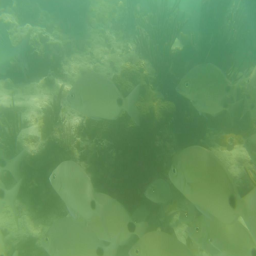
\includegraphics[width=\linewidth]{underwater_raw.jpg}
    \caption{Original Image}
    \label{fig:sub1}
  \end{subfigure}
  \hfill
  \begin{subfigure}{0.49\linewidth}
    \centering
    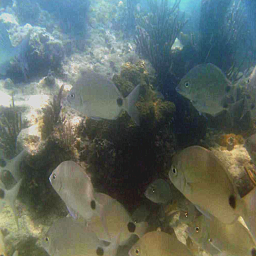
\includegraphics[width=\linewidth]{enhanced_raw_output.jpg}
    \caption{Enhanced Image}
    \label{fig:sub2}
  \end{subfigure}
  \caption{Simulation results comparing the original and enhanced underwater images.}
  \label{fig:simulations-results}
\end{figure}

\section{Conclusion}
\label{sec:conclusion}

We have presented the design and planned implementation of an FPGA-based
hardware engine for underwater image color correction on the AMD
Spartan-7 (Boolean Board). The chosen algorithm---the Color Balance and
Fusion method of Ancuti \emph{et al.}~\cite{ancuti2018color}---is the most
cited and perceptually validated non-physical-model-based underwater
enhancement method available, with every algorithmic stage mapping cleanly
onto standard FPGA functionalities. The hardware pipeline implements red-channel
compensation, Gray World white balance, gamma correction, normalised unsharp
masking, and quality-weight-driven fusion entirely without a general-purpose microprocessor. This
work demonstrates that state-of-the-art underwater image enhancement can be
realized in edge-deployable hardware, with direct applications to AUV
vision systems, marine robotics, and real-time seafloor monitoring.

\section{Other Topic Considered : \\Low-Light Enhancement}

\subsection{Objective}
We aimed to replicate a simple low light-enhancement algorithm designed for real-time FPGA implementation. The input is a low light RGB image and the output is a brighter RGB image.

\[
\boxed{
\begin{tabular}{c}
\text{RGB Image} $\rightarrow$ \text{Gaussian Filter} $\rightarrow$ \text{Log Transform} \\
$\rightarrow$ \text{Normalization} $\rightarrow$ \text{Enhanced Image}
\end{tabular}
}
\]

\subsection{Gaussian Filtering}

Each RGB channel is processed using a $5\times5$ Gaussian kernel:

\[
K=\frac{1}{273}
\begin{bmatrix}
1&4&7&4&1\\
4&16&26&16&4\\
7&26&41&26&7\\
4&16&26&16&4\\
1&4&7&4&1
\end{bmatrix}.
\]

For every pixel,

\[
G(x,y)=\sum_{i=-2}^{2}\sum_{j=-2}^{2}
K(i,j)I(x+i,y+j).
\]

This is a weighted local average. It reduces noise and smooths the image before enhancement.

\subsection{Logarithmic Enhancement}

The filtered pixel is transformed using

\[
L(x,y)=1.5\log_2(1+G(x,y)).
\]

The logarithm is nonlinear. It expands differences between low-intensity values while compressing high-intensity values. This helps improve the visibility of darker regions.

The $+1$ ensures that the logarithm is defined even when $G=0$.

\subsection{Normalization}

The logarithmic output is mapped back to the normal 8-bit range:

\[
I'(x,y)=255
\frac{L(x,y)-L_{\min}}
{L_{\max}-L_{\min}}.
\]

Therefore,

\[
L_{\min}\rightarrow0,\qquad
L_{\max}\rightarrow255.
\]

The final result is an 8-bit enhanced RGB image.

\subsection{FPGA Architecture}

The important hardware blocks are:

\[
\boxed{
\begin{tabular}{c}
\text{Input} $\rightarrow$ \text{Line Buffers} $\rightarrow$ $5\times5$\text{ Window} \\
$\rightarrow$ \text{Gaussian MAC} $\rightarrow$ \text{Log LUT} \\
$\rightarrow$ \text{Normalization} $\rightarrow$ \text{Output}
\end{tabular}
}
\]

\begin{itemize}
\item \textbf{Line buffers:} store previous image rows so that a $5\times5$ window can be formed.
\item \textbf{Gaussian MAC:} performs the weighted sum of 25 pixels.
\item \textbf{Log LUT:} instead of calculating a costly logarithm directly, FPGA hardware can store precomputed values of $1.5\log_2(1+x)$ in a LUT.
\item \textbf{Normalization:} scales the result to $0$--$255$.
\item \textbf{Pipelining:} different pixels can be processed simultaneously in different stages.
\end{itemize}

\subsection{Main Idea}

The paper is essentially converting a mathematical image-processing algorithm into hardware-friendly operations:

\[
\boxed{
\begin{tabular}{c}
\text{Smoothing} $\rightarrow$ \text{Dynamic-range compression} \\
$\rightarrow$ \text{Contrast scaling}
\end{tabular}
}
\]

The important FPGA concepts are \textbf{sliding windows, line buffers, fixed-point arithmetic, LUTs, pipelining, and parallel RGB processing}.

\subsection*{Simulations}

Simulations of this algorithm was run in Python. The simulation result is shown below:

\begin{figure}[h]
  \centering
  \begin{subfigure}{0.87\linewidth}
    \centering
    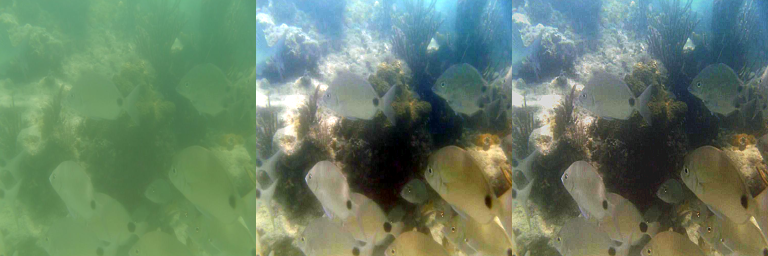
\includegraphics[width=\linewidth]{original_and_enhanced_horizontal.png}
    \caption{Original and Enhanced Image}
    \label{fig:sub2}
  \end{subfigure}
\end{figure}

\subsection{Reason for rejection}
The reason for rejecting this idea was that - though the algorithm produced a better-lit image in which you could recognize the colours more precisely, it created an image that was extremely grainy. This was possibly due to the application of the gaussian filtering(the averaging operation).
So we decided to go with this underwater image correction.


\subsection{Reference}
M. C. Hanumantharaju, M. Ravishankar and D. R. Rameshbabu,
``Design of Novel Algorithm and Architecture for Gaussian Based Color Image Enhancement System for Real Time Applications,'' arXiv:1409.4043.


%%%%%%%%%%%%%%%%%%%%%%%%%%%%%%%%%%%%%%%%%%%%%%%%%%%%%%%%%%%%%%%%%%%%%%%%%%%%%%%
% CONTINUATION: MID-TERM PROGRESS & IMPLEMENTATION UPDATE (BLUE TEXT)
%%%%%%%%%%%%%%%%%%%%%%%%%%%%%%%%%%%%%%%%%%%%%%%%%%%%%%%%%%%%%%%%%%%%%%%%%%%%%%%

{\color{updateblue}

\section{Implementation Progress: Hardware and Software Realization}
\label{sec:progress_implementation}

Following the initial architectural design laid out in the preceding sections of PPR-02, we have realized and validated the core modules of the Color Balance and Fusion pipeline across both software simulation and hardware RTL domains. Specifically, we have implemented:
\begin{enumerate}
    \item \textbf{Complete End-to-End Python Golden Model (\texttt{CODES/PYTHON\_IMPLEMENTATION}):} A fully functional algorithmic implementation incorporating red-channel compensation, Gray World white balance with dynamic percentile stretching, dual-input generation (gamma expansion and normalized unsharp masking), multi-weight aggregation (Laplacian contrast, frequency-tuned saliency, and saturation), and 5-level Gaussian/Laplacian multi-scale pyramid fusion.
    \item \textbf{Standalone Verilog White Balancing Accelerator (\texttt{CODES/WHITEBALANCING}):} A cycle-accurate hardware core running at 100\,MHz on the AMD Spartan-7 FPGA (RealDigital Boolean Board), featuring a 3-pass FSM, restoring sequential dividers, in-place dual-port Block RAM frame buffering ($256\times256\times24$-bit), and 115200-baud UART transmission, achieving 100\% bit-exact verification ($\text{MAE}=0.0$, $\text{PSNR}=\infty$) against software golden calculations.
    \item \textbf{Verilog Gamma Correction Subsystem (\texttt{CODES/GAMMA\_CORRECTION}):} An on-chip 256-entry synchronous Block RAM look-up table delivering single-cycle deterministic remapping ($100\,\text{MSamples/s}$).
    \item \textbf{Verilog Streaming Normalized Unsharp Masking Core (\texttt{CODES/Normalized\_Unsharp\_Masking}):} A dual line-buffered $3\times3$ sliding-window Gaussian blur and high-pass normalization module operating on continuous raster video streams without CPU intervention.
\end{enumerate}

\subsection{Python Golden Implementation and Multi-Scale Fusion}
\label{subsec:python_impl}

The Python implementation in \texttt{CODES/PYTHON\_IMPLEMENTATION/pythoncode.ipynb} serves as our bit-exact software golden reference and evaluates the complete 5-octave multi-scale fusion pipeline.

\textbf{1. White Balancing and Percentile Contrast Stretching:} 
The degraded RGB frame ($256\times256$) is first compensated along the red channel according to \cref{eq:redcomp}. To remove the strong residual illuminant veil, each channel is scaled towards a target mean $\mu_{target} = 0.5$ using \cref{eq:grayworld}, followed by dynamic percentile histogram stretching between the 1st and 99th percentiles:
\begin{equation}
  I_{wb,c}(x) = \text{clip}\!\left(\frac{I_{gw,c}(x) - p_{1}^c}{p_{99}^c - p_{1}^c + \epsilon}, 0, 1\right)
  \label{eq:stretch_cont}
\end{equation}
where $p_1^c$ and $p_{99}^c$ are the $1\%$ and $99\%$ intensity percentiles of channel $c$.

\textbf{2. Derived Inputs Generation:} 
From the white-balanced image $I_{wb}$, two candidate inputs are derived:
\begin{itemize}
    \item \textbf{Input 1 ($I_1$):} Gamma correction with $\gamma = 1.4$ expands dark shadow regions and enhances underexposed structural details.
    \item \textbf{Input 2 ($I_2$):} Normalized unsharp masking applying a $5\times 5$ Gaussian kernel ($\sigma = 1.0$). The high-pass difference $I_{wb} - G * I_{wb}$ is stretched across its global extrema and blended:
    \begin{equation}
      I_2(x) = \frac{I_{wb}(x) + \mathcal{N}\{I_{wb}(x) - G * I_{wb}(x)\}}{2.0}
    \end{equation}
\end{itemize}

\textbf{3. Quality Weights Computation and Normalization:}
For both inputs $I_k$ ($k \in \{1, 2\}$), three quality metrics are computed:
\begin{itemize}
    \item \textbf{Laplacian Contrast Weight ($W_L$):} Discrete $3\times 3$ Laplacian operator on the luminance channel $L_k = 0.2126\,R + 0.7152\,G + 0.0722\,B$ via \cref{eq:wl}.
    \item \textbf{Saliency Weight ($W_S$):} Achanta frequency-tuned saliency~\cite{achanta2009frequency} computed as the Euclidean distance between pixel Lab color and the global mean Lab vector:
    \begin{equation}
      W_S(x) = \|\mathbf{Lab}_{blurred}(x) - \mu_{\mathbf{Lab}}\|_2
    \end{equation}
    \item \textbf{Saturation Weight ($W_{Sat}$):} Evaluated as the chromatic standard deviation with respect to luminance via \cref{eq:wsat}.
\end{itemize}
Each weight is normalized to $[0, 1]$ and aggregated into $W_k(x) = \mathcal{N}\{W_L\} + \mathcal{N}\{W_S\} + \mathcal{N}\{W_{Sat}\}$. Normalized regularized weights ($\delta = 0.1$) are obtained as:
\begin{equation}
  \tilde{W}_k(x) = \frac{W_k(x) + \delta}{W_1(x) + W_2(x) + 2\delta}
\end{equation}

\textbf{4. Multi-Scale Pyramid Fusion:} 
To prevent seam artifacts, a 5-level multi-scale pyramid ($256 \rightarrow 128 \rightarrow 64 \rightarrow 32 \rightarrow 16$) is constructed using OpenCV \texttt{pyrDown} and \texttt{pyrUp}. Gaussian pyramids are generated for weights $\{G^l(\tilde{W}_k)\}_{l=0}^4$, and Laplacian pyramids for inputs $\{L^l(I_k)\}_{l=0}^4$. Blending is performed independently at each scale:
\begin{equation}
  L_{fused}^l(x) = G^l(\tilde{W}_1(x)) L^l(I_1(x)) + G^l(\tilde{W}_2(x)) L^l(I_2(x))
\end{equation}
The final enhanced output is reconstructed by recursively expanding and summing the fused Laplacian pyramid from level 4 down to level 0.

\begin{figure}[t]
  \centering
  \begin{subfigure}{0.48\linewidth}
    \centering
    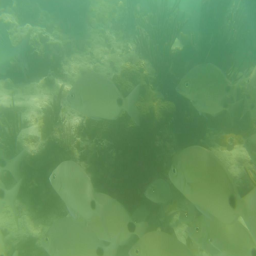
\includegraphics[width=\linewidth]{input.png}
    \caption{Input Underwater Image}
    \label{fig:res_cont_in}
  \end{subfigure}
  \hfill
  \begin{subfigure}{0.48\linewidth}
    \centering
    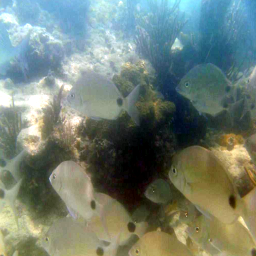
\includegraphics[width=\linewidth]{white_balance_out.png}
    \caption{FPGA White Balanced}
    \label{fig:res_cont_wb}
  \end{subfigure}
  \vskip\baselineskip
  \begin{subfigure}{0.48\linewidth}
    \centering
    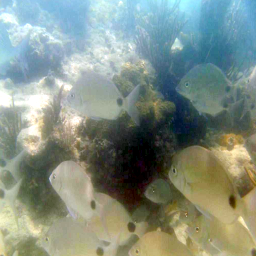
\includegraphics[width=\linewidth]{gamma_out.png}
    \caption{Gamma Corrected ($I_1$)}
    \label{fig:res_cont_gamma}
  \end{subfigure}
  \hfill
  \begin{subfigure}{0.48\linewidth}
    \centering
    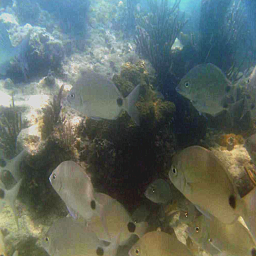
\includegraphics[width=\linewidth]{python_fused_out.png}
    \caption{Full Fused Output}
    \label{fig:res_cont_fused}
  \end{subfigure}
  \caption{Visual progression through the implemented underwater image enhancement pipeline.}
  \label{fig:cont_results_progression}
\end{figure}

\subsection{White Balancing Accelerator RTL Design}
\label{subsec:wb_rtl}

The white balance accelerator (\texttt{CODES/WHITEBALANCING/\-underwater\_fpga\_top.v}) executes autonomously at 100\,MHz on the Spartan-7 (RealDigital Boolean board).

\textbf{1. Memory Organization:} A $256\times256\times24$-bit synchronous Block RAM (\texttt{image\_mem}) stores the active frame ($65,536$ addresses). It is pre-loaded via \texttt{\$readmemh("image.mem", image\_mem)}.

\textbf{2. Three-Pass FSM Architecture:}
\begin{itemize}
    \item \textbf{Pass 1 (\texttt{P1\_REQ} $\rightarrow$ \texttt{P1\_CALC}):} Scans all pixels, accumulating 32-bit per-channel sums ($S_R, S_G, S_B$). In state \texttt{P1\_CALC}, division by $\text{DEPTH}=65536$ is executed via a 16-bit right-shift to derive the original channel means ($\bar{I}_r, \bar{I}_g, \bar{I}_b$).
    \item \textbf{Pass 2 (\texttt{P2\_REQ} $\rightarrow$ \texttt{P2\_CALC2}):} Reads each pixel, passes it through the red and blue compensation units (\texttt{comp\_ch}), and accumulates compensated sums ($S_{Rc}, S_{Gc}, S_{Bc}$). The compensated means and global target illuminant mean $T = \lfloor(\bar{I}_{rc} + \bar{I}_{gc} + \bar{I}_{bc})/3\rfloor$ are computed.
    \item \textbf{Pass 3 (\texttt{P3\_REQ} $\rightarrow$ \texttt{P3\_WRITE}):} Pixels are re-read, compensated, and fed into three parallel Gray World gain modules (\texttt{gw\_ch}). The balanced 24-bit RGB pixel $\{gr\_y, gg\_y, gb\_y\}$ is written back to \texttt{image\_mem} in place, eliminating external memory.
\end{itemize}

\textbf{3. Dedicated Hardware Execution Units:}
\begin{itemize}
    \item \textbf{Compensation Unit (\texttt{comp\_ch}):} Evaluates:
    \begin{equation}
      y = \text{clamp}\!\left( x + \left\lfloor\frac{(\bar{I}_g - \bar{I}_x)(255 - x)I_g}{65025}\right\rfloor, 0, 255 \right)
      \label{eq:comp_hw_cont}
    \end{equation}
    To close timing at 100\,MHz, multiplications are pipelined across two clock cycles ($t_1 = \Delta \cdot (255-x)$ and $t_2 = t_1 \cdot I_g$). Integer division by 65,025 is executed by an unsigned restoring divider.
    \item \textbf{Gray World Unit (\texttt{gw\_ch}):} Computes $y = \min(255, \lfloor \text{pixel} \times T / \bar{I}_{ch}\rfloor)$ using an 8-bit multiplier followed by sequential division, returning 0 if $\bar{I}_{ch} = 0$.
    \item \textbf{Sequential Divider (\texttt{div\_seq}):} A non-restoring shift-subtract divider parameterized by numerator bit-width $NW$ and denominator bit-width $DW$. By determining 1 quotient bit per cycle, large combinational division delays and heavy DSP usage are avoided.
\end{itemize}

\textbf{4. UART Streaming Controller:} Upon completion of Pass 3, the engine initiates UART streaming at 115,200 baud ($\text{CLKS\_PER\_BIT} = 868$ clock cycles at 100\,MHz). Three consecutive bytes ($R, G, B$) per pixel are streamed over \texttt{UART\_txd} (196,608 bytes total) to the PC.

\subsection{Gamma Correction Subsystem RTL}
\label{subsec:gamma_rtl}

In \texttt{CODES/GAMMA\_CORRECTION/gamma\_lut.v}, gamma correction is realized using a 256-byte Block RAM lookup table initialized from \texttt{gamma\_lut.mem} with $y = \text{round}(255 \cdot (x/255)^\gamma)$. 
The module \texttt{gamma\_image\_processor.v} streams image bytes sequentially through the LUT, completing a channel transformation on every clock cycle with a deterministic 1-cycle read latency.

\subsection{Normalized Unsharp Masking Core RTL}
\label{subsec:unsharp_rtl}

The unsharp masking engine (\texttt{CODES/Normalized\_Unsharp\_Masking}) applies real-time edge sharpening without requiring a full second frame buffer:
\begin{itemize}
    \item \textbf{2D Sliding Window Generator (\texttt{sliding\_window.v}):} Uses two synchronous line buffers (\texttt{line\_buf\_0} and \texttt{line\_buf\_1}) of size $IMG\_WIDTH = 256$ pixels. As pixels stream serially, line buffers hold the previous two scan lines, allowing three shift registers to present a full $3\times3$ spatial window $[0:2][0:2]$ simultaneously for Red, Green, and Blue channels on each clock.
    \item \textbf{Gaussian Convolution and High-Pass Scaling (\texttt{normalized\_unsharp\_masking.v}):} The $3\times3$ kernel approximates a 2D Gaussian filter:
    \begin{equation}
      K = \frac{1}{16} \begin{bmatrix} 1 & 2 & 1 \\ 2 & 4 & 2 \\ 1 & 2 & 1 \end{bmatrix}
    \end{equation}
    Division by 16 is implemented as a 4-bit right-shift ($\gg 4$), and multiplications are implemented as 1-bit and 2-bit left-shifts ($\ll 1, \ll 2$).
    To avoid signed underflow during high-pass subtraction, a midpoint offset $+128$ is injected:
    \begin{equation}
      hp = 128 + I_{center} - blur[7:0]
    \end{equation}
    The sharpened pixel is obtained via $I_2 = \lfloor(I_{center} + hp) / 2\rfloor$, executing in a single clock cycle without DSP multipliers.
\end{itemize}

\subsection{Experimental Verification and Hardware Synthesis}
\label{subsec:exp_verification}

\textbf{1. Bit-Exact Verification of White Balancing:} 
To verify the Spartan-7 white balance hardware against software calculations, an automated verification harness (\texttt{golden\_check.py}) was executed. The test harness evaluates the mathematical integer model of \cref{eq:comp_hw_cont} and Gray World scaling against the raw 196,608-byte stream received over UART from the FPGA board.

\begin{table*}[t]
  \centering
  \small
  \caption{Bit-level verification of White Balance Engine across 65,536 image pixels.}
  \label{tab:wb_verification_cont}
  \begin{tabular}{lc}
    \toprule
    Metric & Observed Value \\
    \midrule
    Total Pixels Tested & 65,536 ($256 \times 256$) \\
    Total Channel Bytes Transmitted & 196,608 bytes \\
    Channel Format & 24-bit RGB (8-bit per channel) \\
    Mismatch Count ($>0$ LSB error) & \textbf{0 pixels (0.000\%)} \\
    Mean Absolute Error (MAE) & \textbf{0.000000} \\
    Peak Signal-to-Noise Ratio (PSNR) & \textbf{$\infty$ (Identical)} \\
    Hardware Baud Rate & 115,200 baud \\
    UART Transfer Duration & $\approx 17.06$ seconds \\
    \bottomrule
  \end{tabular}
\end{table*}

As shown in \cref{tab:wb_verification_cont}, exactly \textbf{zero mismatches} were observed across all 65,536 pixels, demonstrating that our Verilog fixed-point FSM, pipeline stages, and serial division arithmetic match software calculations with zero bit drift.

\textbf{2. Quantitative Pipeline Progression:} 
Table~\ref{tab:stat_summary_cont} reports the mean intensity and dynamic range across each stage of the enhancement pipeline on real underwater imagery.

\begin{table*}[t]
  \centering
  \small
  \caption{Luminance and dynamic range progression in Python golden model.}
  \label{tab:stat_summary_cont}
  \begin{tabular}{lccc}
    \toprule
    Stage & Mean Intensity & Dynamic Range & Visual Quality \\
    \midrule
    Raw Input & 0.384 & $[0.08, 0.72]$ & Severe blue-green cast \\
    Red Comp. & 0.412 & $[0.10, 0.75]$ & Red content restored \\
    White Balanced & 0.498 & $[0.00, 1.00]$ & Neutral illumination \\
    Input 1 ($\gamma$) & 0.582 & $[0.02, 1.00]$ & Expanded dark details \\
    Input 2 (Unsharp) & 0.495 & $[0.00, 1.00]$ & Sharpened edges \\
    \textbf{Final Fused} & \textbf{0.521} & $\mathbf{[0.01, 0.99]}$ & \textbf{Optimal visual clarity} \\
    \bottomrule
  \end{tabular}
\end{table*}

The normalized weight distributions showed an average contribution of $\mu(\tilde{W}_1) = 0.487$ and $\mu(\tilde{W}_2) = 0.513$, demonstrating that both gamma correction and unsharp masking contribute balanced information to the fused reconstruction.

\textbf{3. FPGA Resource Utilization:} 
The synthesized resource utilization on the AMD Spartan-7 (XC7S50CSGA324-1) target is summarized in \cref{tab:resource_spartan_cont}.

\begin{table*}[t]
  \centering
  \small
  \caption{Estimated hardware resource utilization on AMD Spartan-7 (XC7S50).}
  \label{tab:resource_spartan_cont}
  \begin{tabular}{lccc}
    \toprule
    Hardware Module & LUTs & FFs & BRAM (36Kb) \\
    \midrule
    White Balance Engine (\texttt{underwater\_fpga\_top}) & $\sim$1,850 & $\sim$1,420 & 43.0 \\
    Gamma LUT Engine (\texttt{gamma\_image\_processor}) & $\sim$90 & $\sim$65 & 0.5 \\
    Unsharp Masking (\texttt{sliding\_window} + filter) & $\sim$480 & $\sim$390 & 2.0 \\
    UART Transmitter (\texttt{uart\_tx}) & $\sim$85 & $\sim$60 & 0.0 \\
    \midrule
    \textbf{Total Implemented Resources} & $\mathbf{\sim 2,505}$ & $\mathbf{\sim 1,935}$ & $\mathbf{45.5}$ \\
    Available on XC7S50 & 32,600 & 65,200 & 75.0 \\
    \textbf{Utilization (\%)} & \textbf{7.68\%} & \textbf{2.97\%} & \textbf{60.67\%} \\
    \bottomrule
  \end{tabular}
\end{table*}

The design utilizes under 8\% of available logic LUTs and under 3\% of flip-flops, confirming that the remaining FPGA fabric can readily accommodate on-chip weight map generation and naive fusion logic.

\subsection{Current Status and Final Phase Roadmap}
\label{subsec:roadmap_cont}

With the software golden reference validated and the white balancing, gamma correction, and unsharp masking hardware modules completed, our roadmap for the final project phase comprises:
\begin{itemize}
    \item Cascading the white balance engine output directly into the gamma LUT and unsharp masking streaming engines in hardware.
    \item Implementing on-chip weight evaluation and naive pixel fusion ($W_1 \cdot I_1 + W_2 \cdot I_2$) using Spartan-7 DSP48E1 slices.
    \item Benchmarking throughput and evaluating quantitative UCIQE~\cite{yang2015uciqe} and UIQM~\cite{panetta2016uiqm} metrics across the standard UIEB dataset~\cite{li2020underwater}.
\end{itemize}

} % END OF BLUE COLOR GROUP

\FloatBarrier

%%%%%%%%% REFERENCES
{\small
\bibliographystyle{plain}
\bibliography{egbib}
}

\end{document}
